\documentclass{article}

\usepackage[utf8]{inputenc}
\usepackage[ngerman]{babel}
\usepackage[hidelinks]{hyperref}
\usepackage{graphicx}
\usepackage{tabularx}
\usepackage{float}
\usepackage[style=ieee,backend=biber]{biblatex}
\addbibresource{bib/literature}
\usepackage{csquotes}

\begin{document}

\section{Example Section}\label{section_one}

Citation \cite{aharonov2008quantum}.

Reference to \autoref{section_one}

\begin{figure}[H]
  \centering
  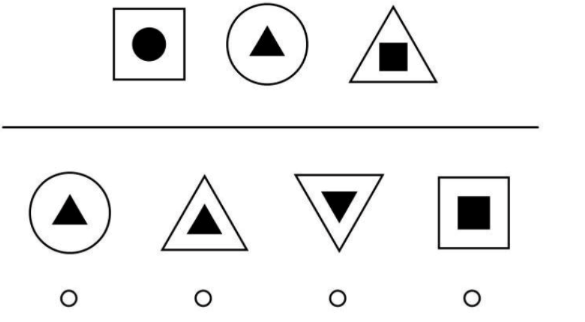
\includegraphics[scale=.5]{figures/example_figure.png} \\
  \caption{Example Figure}\label{fig:example_figure}
\end{figure}

\begin{table}[htbp]
  \centering
  \begin{tabularx}{\textwidth}{| p{1cm} | X | p{6cm} |}
    \hline
      1 & Lorem
        & Ipsum \\ \hline
      2 & Dolorum
        & Est \\ \hline
  \end{tabularx}
  \caption{Example Table}
\end{table}

% **************************************
% Table of figure/tables & bibliography
% **************************************
\listoffigures
\listoftables
\printbibliography
\end{document}
